\chapter[Introdução]{Introdução}

Neste capítulo, é introduzido o trabalho de conclusão de curso. O capítulo está dividido em seções que estão dispostas da seguinte maneira: na seção 1.1 é contextualizado de forma resumida o que são as metodologias ativas de aprendizado até chegar no foco que é a metodologia \textit{Team Based Learning}; na seção 1.2 é apresentado a problemática; na seção 1.3 é apresentado a justificativa; na seção 1.4 os objetivos; na seção 1.5 é apresentado a metodologia de pesquisa e desenvolvimento e por fim, na seção 1.6 é apresentado a organização do trabalho.


\section{Contextualização}

A educação está em um impasse diante das várias mudanças acontecendo na sociedade atual. As instituições que ensinam e avaliam a todos de forma igual e exigem resultados previsíveis, ignoram o fato que hoje vivemos em uma sociedade do conhecimento. Essa sociedade é baseada em competências cognitivas, pessoais e sociais, que não se adquirem da forma convencional e que exigem proatividade, visão, personalização, colaboração e empreendedorismo \cite{moran}.

Na época em que o acesso à informação era difícil, fazia sentido os métodos tradicionais, que privilegiam a transmissão de informação pelos professores. Com a chegada da internet podemos aprender em qualquer lugar, a qualquer hora e com muitas pessoas diferentes. Essa mescla, entre sala de aula e ambientes virtuais é fundamental para abrir a escola para o mundo e trazer o mundo para dentro da escola \cite{moran}.

Dentro dessa era tecnológica em que vive a sociedade do conhecimento, o software faz parte do cotidiano das pessoas, podendo ser encontrado em hospitais, escolas,  atividades de lazer e de segurança, entre outros.  No entanto, a produção de software ainda enfrenta uma série de desafios, como redução de custos, cumprimento de prazos e alta obtenção de qualidade do produto final \cite{silva}.

Diante disso a Engenharia de Software apareceu para melhorar a sistematização do desenvolvimento de software, que deveria ser tratado como engenharia e não como arte. Desta  forma, a ideia foi propor a utilização de métodos, ferramentas e técnicas para a produção de software confiável, correto e entregue, respeitando os prazos e custos definidos \cite{soares}.

Não é de hoje que o mercado de engenharia exige dos seus profissionais algumas competências importante, como: capacidade de trabalho em equipe, análise de dados, resolução de problemas reais \cite{davis}. As metodologias ativas de aprendizagem têm como objetivo preencher essas lacunas que o mercado exige dos alunos para que esses se sintam melhor preparados para o mercado.

Apesar de pouco conhecidas, as metodologias ativas de aprendizagem já vêm sendo aplicadas de forma indireta pelos professores por meio de projetos, resolução de problemas e outros meios de ensinar e aprender que podem ser considerados como um tipo de metodologia ativa \cite{moran}.

Silberman, citado por \cite{barbosa} modificou, com suas palavras um provérbio chinês dito pelo filósofo Confúcio para facilitar o entendimento de métodos ativos de aprendizagem, que diz:

\begin{quote}
“O que eu ouço, eu esqueço; o que eu ouço e vejo, eu me lembro; o que eu ouço, vejo e pergunto ou discuto, eu começo a compreender; o que eu ouço, vejo, debato e faço, eu aprendo desenvolvendo conhecimento e habilidade; o que eu ensino para alguém, eu domino com maestria.”
\end{quote}

Essa citação, com a modificação de Silberman, resume a teoria por trás das metodologias ativas de aprendizagem. Se o ensino englobar as atividades de ouvir, ver,  perguntar, discutir, fazer e ensinar, estamos no caminho da aprendizagem ativa \cite{barbosa}.

Existem hoje diversas metodologias ativas de aprendizagem, por exemplo, o \textit{Team-Based Learning} ou TBL é uma metodologia de aprendizagem colaborativa, já o \textit{Problem-Based Learning}, conhecida como PBL, é mais focada na resolução de problemas complexos com um toque ainda na abordagem pedagógica de ensino tradicional, como slides, provas e etc \cite{cabrera}. O \textit{Project-Based Learning}, tem como base a resolução de desafios por meio de projetos. Além disso pode-se contar com o apoio de um método ativo bastante atual chamado Sala de Aula Invertida que nada mais é  do que substituir a maioria das aulas por conteúdos virtuais para que o tempo em sala seja otimizado \cite{moran}.

O principal foco deste trabalho é na metodologia ativa de aprendizado TBL, o qual  implementa o construtivismo e dá ênfase no papel do aluno como mestre de suas próprias experiências educacionais. Eles saem de agente passivo do conhecimento para um agente ativo \cite{gomez}.

\section{Problemática}

A maioria dos casos de uso do TBL utiliza-se de ferramentas de CMC (\textit{Computer Mediated Communication}) como fóruns de discussão, chats entre outros meios de comunicação eletrônicos como Facebook \cite{alhomod}, Blackboard, Moodle, Wiki ou Google Drive \cite{awatramani}, entre outras tecnologias web \cite{kam}. Às vezes, utilizam até mais de uma dessas ferramentas juntas.

Mais especificamente, as ferramentas de comunicação fornecem um meio que permite que grupos de alunos troquem idéias e opiniões e compartilhem informações a qualquer hora e em qualquer lugar. Os principais benefícios do uso de CMC são a conveniência, a independência do lugar, do tempo e o potencial para que os usuários se tornem parte de uma comunidade virtual \cite{berge}. Porém, essas ferramentas são uma extensão do uso do TBL e não uma forma de automatizar o uso do mesmo.

Um excelente exemplo de uso de ferramenta de CMC é o \textit{Moodle}, ela é uma boa ferramenta para disponibilizar materiais e notas, além de ter um pequeno fórum para discussão. Porém, muitas vezes esses tipos de ferramentas deixam a desejar em vários aspectos, por exemplo, ela não calcula as notas dos alunos e dos grupos automaticamente. Este cálculo é bem trabalhoso de se fazer já que o TBL é feito por pontuação e não por menção como é feito nas universidades e escolas, ele não gera relatórios para o professor saber qual é o tema que está gerando mais dúvidas entre os alunos, entre outros aspectos.

Além disso temos alguns problemas relacionados as metodologias tradicionais, estão definidas no diagrama de espinha de peixe da figura \ref{fig:fishbone}

\begin{figure}[H]
	\centering
  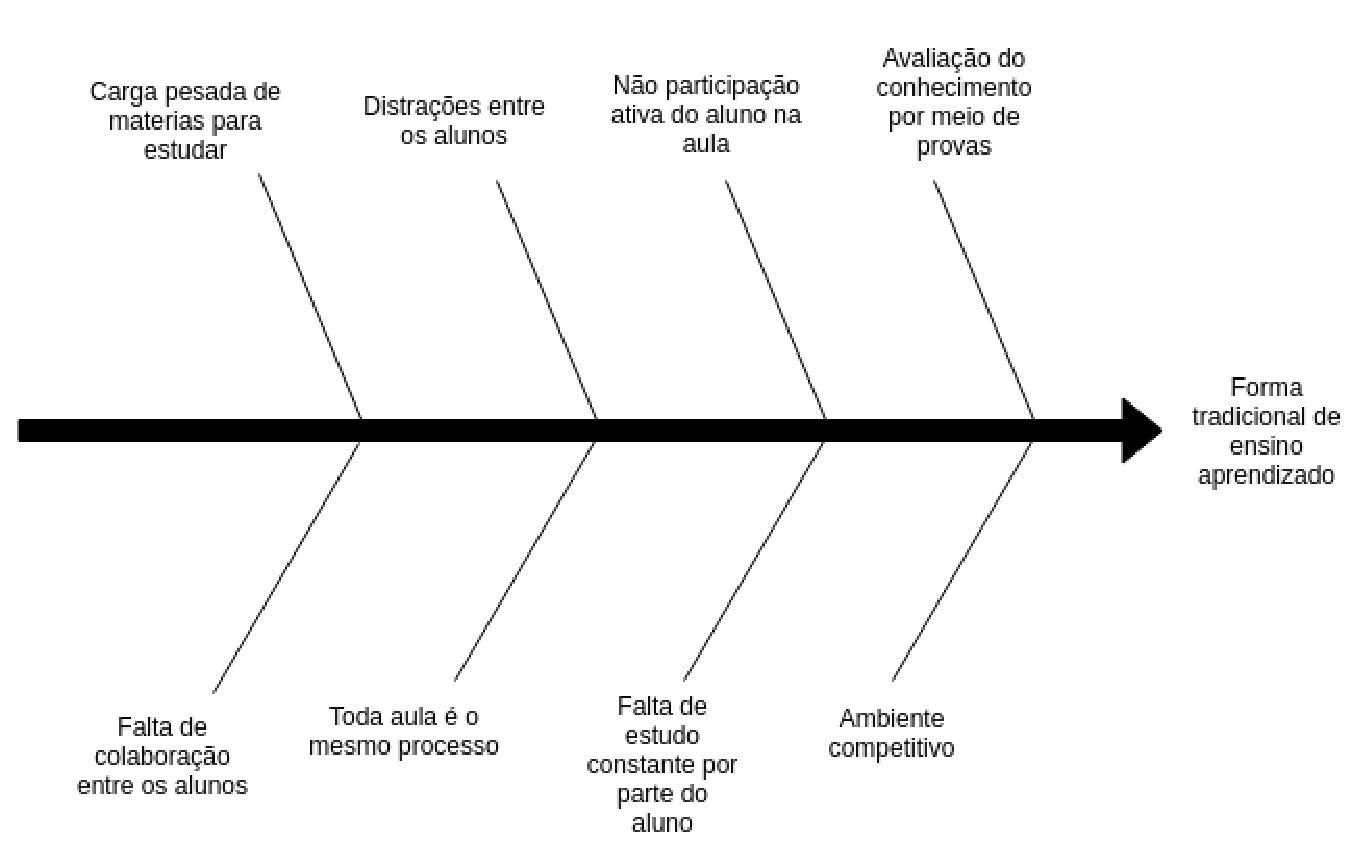
\includegraphics[keepaspectratio=true,scale=0.5]{figuras/fishbone.eps}
  \caption[Diagrama Espinha de Peixe]{Diagrama Espinha de Peixe. Fonte: Autor}
	\label{fig:fishbone}
\end{figure}

Com isso temos a seguinte questão: A automatização da metodologia ativa de aprendizado por uma ferramenta tornaria mais fácil a sua implantação em sala de aula? Tornando o processo mais prazeroso, tanto para o aluno quanto para o professor.

\section{Justificativa}

Procurando colaborar com essa problemática, o presente trabalho propôs a construção de uma plataforma para automatizar todo o processo da metodologia ativa de aprendizado: Team Based Learning, e com isso validar se a ferramenta estaria sendo efetiva no seu propósito.

\section{Objetivo}

O objetivo deste trabalho é a implementação da plataforma de gerenciamento da metodologia ativa de aprendizado: \textit{Team Based-Learning}, chamada PGTBL, para automatizar o uso dessa metodologia no ambiente acadêmico da FGA. Temos como objetivos específicos:

\begin{itemize}
  \item Estudar o contexto do Team Based Learning;
  \item Especificar os requisitos;
  \item Adaptar a metodologia ágil para as necessidades do projeto;
  \item Desenvolver a ferramenta e testá-la em um contexto real.
  \item Coletar feedback dos alunos comparando a utilização da metodologia antes e depois da ferramenta.
\end{itemize}

\section{Metodologia}

A metodologia utilizada para a implementação da ferramenta é a metodologia ágil com adaptações para a utilização do SCRUM, XP e SAFe para ser utilizado por um único desenvolvedor. Além disso, a ferramenta terá acesso livre para contribuições externas durante seu desenvolvimento, aplicando todas as boas práticas definidas na comunidade \textit{Open Source}.

Como base de sustentação do trabalho, foi realizada uma pesquisa bibliográfica com o intuito de reunir as informações e dados que servirão de base para a construção da ferramenta, utilizando como banco de dados a Scopus e o Google Acadêmico, além de documentações ou sites oficiais de ferramentas ou metodologias.

\section{Organização do Trabalho}

O trabalho está organizado da seguinte forma: No Capítulo 2 é apresentado o referencial teórico quanto ao contexto do TBL, gerenciamento utilizando scrum, xp e safe, qualidade de software utilizando como base o \textit{Goal Question Metric} (GQM) para coleta de métricas e alguns conceitos de testes, devops e software livre. No Capítulo 3 é apresentado a metodologia de desenvolvimento, ou seja, será apresentado passo a passo o processo na qual o desenvolvimento será realizado e a metodologia do trabalho de conclusão de curso (TCC). No Capítulo 4 é apresentado a proposta de trabalho que terá uma visão geral do produto a ser desenvolvido, além de algumas informações técnicas e de gerenciamento como \textit{Roadmap}, ferramentas, Estrutura análitica do projeto (EAP), arquitetura e requisitos iniciais. E por último, temos as Considerações Finais na qual terá um resumo geral do que foi falado, e o que se pode esperar do projeto no futuro.
